\chapter{Introduzione al ML}
\label{Capitolo 1}

%----------------------------------------------------------------------------------------
%	SECTION 
%----------------------------------------------------------------------------------------
\section{L'idea alla base}
Un \textbf{sistema di apprendimento automatico} ricava da un insieme di dati
una conoscenza non fornita a priori al fine di creare dei modelli in grado di \textit{soddisfarli}. 
L'idea è quella di creare un modello in grado di approssimare il più possibile i dati proposti 
in modo tale da trovare una correlazione tra essi. In
quest'ottica bisogna mediare tra \textbf{fit} e \textbf{complessità}. Ogni
sistema dovrà cercare di mediare tra questi due aspetti, dove un \textit{fit}
migliore comporta alta \textit{complessità}. Si ha sempre il rischio di \textbf{overfitting} 
\footnote{In statistica e in informatica, si parla di overfitting (in italiano: adattamento eccessivo, sovradattamento) quando un modello statistico molto complesso si adatta ai dati osservati (il campione) perché ha un numero eccessivo di parametri rispetto al numero di osservazioni.
Un modello assurdo e sbagliato può adattarsi perfettamente se è abbastanza complesso rispetto alla quantità di dati disponibili.
Si sostiene che l'overfitting sia una violazione del principio del rasoio di Occam. }.\\
Definiamo alcuni concetti base:
\begin{itemize}
  \item \textbf{Task (\textit{T})}: il compito da apprendere. È più facile
  apprendere attraverso esempi che codificare conoscenza o definire alcuni
  compiti. Il comportamento della macchina in un ambiente può essere
  diverso da quello desiderato a causa della mutabilità di quest'ultimo, ed è più
  semplice cambiare gli esempi piuttosto che ridisegnare un intero sistema. 
  \item \textbf{Performance (\textit{P})}: la misura della bontà
  dell'apprendimento.
  \item \textbf{Experience (\textit{E})}: l'esperienza sui cui basare
  l'apprendimento. Il tipo di esperienza scelto può variare di molto il risultato e
  il suo successo.
\end{itemize}
In merito alle parti ``software'' distinguiamo:
\begin{itemize}
  \item \textbf{Learner}: la parte di programma che impara dagli esempi in modo
  automatico.
  \item \textbf{Trainer}: il \textit{dataset (o Training Set)} che fornisce esperienza al
  \textit{learner}.
\end{itemize}
Durante l'\textbf{apprendimento} si analizzano gli esempi dati in ingresso al fine di generare un modello che li soddisfi.\\
Approfondiamo il discorso relativo all'\textit{esperienza}. Innanzitutto nel
momento della scelta bisogna valutare la rappresentatività dell'esperienza. 
Oltre ad apprendere, il \textit{learner} ha la facoltà di controllare e manipolare la propria esperienza:
\begin{itemize}
  \item L'esperienza può essere fornita al learner senza che esso possa
  interagire.
  \item Il learner può porre domande su quegli esempi che non risultano chiari. 
\end{itemize}
\textbf{L'esperienza DEVE essere presentata in modo causale.}\\
Esistono due tipi di esperienza:
\begin{enumerate}
  \item \textbf{Diretta}: dove il learner può acquisire informazioni utili
  direttamente dagli esempi o dover inferire indirettamente da essi
  l’informazione necessaria.
  \item \textbf{Indiretta}
\end{enumerate}
\newpage
%----------------------------------------------------------------------------------------
%	SECTION 
%----------------------------------------------------------------------------------------
\section{Terminologia}
\begin{shaded}
  \begin{itemize}
  
    \item $x\in X$, \textbf{istanza}: un singolo ``oggetto'' preso dallo
    \textbf{spazio delle istanze}. Ogni \textbf{istanza} è rappresentata tramite
    un \textbf{vettore di attributi unici} (un attributo per posizione del
    vettore). In termini probabilistici questo equivale a un \textit{evento elementare}.
    
    \item $X$, \textbf{spazio delle istanze}: ovvero la collezione di tutte le
    possibili istanze utili per qualche compito di \textit{learning}. 
    In termini statistici lo \textit{spazio delle istanze} non è altro che lo 
    \textbf{spazio campionario} \footnote{Insieme di tutti i possibili eventi elementari.}
    
    \item $c$, \textbf{concetto}, $c\subseteq X$: ovvero un sottoinsieme dello \textit{spazio delle istanze} che descrive una \textit{classe} d'istanze alla quale siamo interessati per costruire un modello di \textit{machine learning}. In pratica raccolgo quel sottoinsieme d'istanze che mi garantiscono, per esempio, uno o più attributi validi al mio modello. La nozione statistica equivalente è quella di \textit{evento} (ovvero un sottoinsieme dello \textit{spazio campione}).\\ 
    Si ha quindi che, preso un concetto $A\subseteq X$:
    \[f_A:X\to\{0,1\}\]
    
    Si ottiene: 
    
    \[f_a(x)=
      \begin{cases}
        1& \mbox{ se } x\in A\\
        0& \mbox{ altrimenti}
      \end{cases}
    \]
    
    \item $(x, f(x))$, \textbf{esempio}: Ovvero un'istanza etichettata con la sua classe di appartenenza. La funzione $f$ è detta \textbf{funzione target}.
    
    \item $D=\{(x_1,f(x_1)),\ldots,(x_n,f(x_n))\}$, \textbf{Training Set}:
    ovvero è la raccolta degli esempi. Qualora si avesse a che fare con un \textit{training non supervisionato} si avrebbe:
    $D=\{x_1,\ldots,x_n\}$
    
    \item \textbf{Ipotesi (o Modello)}, $h\subseteq X$: Essa rappresenta una possibile soluzione al problema. Normalmente simboleggiata da un vettore booleano dove ogni elemento di esso si riferisce a un attributo.
    \begin{itemize}
        \item \textbf{Ipotesi $h$}: ovvero una congiunzione (\textb{$$\land$}) di vincoli sugli
    attributi. Tale ipotesi è \textbf{consistente}, ovvero è coerente con tutti gli esempi.
    \item \textbf{soddisfazione di un'ipotesi}: un'istanza $x$ soddisfa
    un'ipotesi $h$ sse tutti i vincoli espressi da $h$ sono soddisfatti dai
    valori di $x$ e si indica con:
    \[h(x)=1\]
    \begin{esempio}
      Avendo:
      \[x=\langle S,W,N,S,W,S\rangle \mbox{ \textnormal{e}
        }h=\langle S,?,?,S,?,S\rangle\]
      posso dire che $x$ soddisfa $h$.\\
      se invece ho che:
      \[h=\langle S,?,?,\emptyset,?,S\rangle\]
      posso dire che $x$ non soddisfa $h$.
    \end{esempio} 
    \end{itemize}
    
    \item $H$, \textbf{spazio delle ipotesi (spazio dei Modelli)}: insieme d'ipotesi.
    
    
    \item $\{(x_1',f(x_1')),\ldots,(x_n',f(x_n'))\}$, \textbf{test}
    
    
    \item un \textbf{Modello di machine learning} è
    quindi l'\textit{ipotesi migliore}. Questo \textbf{modello predittivo} viene
    addestrato tramite il \textit{training set} e servirà per inferire nuove
    informazioni mai state osservate nel \textit{training set}. 
    
    
    \item \textbf{Linguaggio delle ipotesi}: è il linguaggio che definisce lo
    \textit{spazio delle ipotesi / modelli}
    \begin{esempio}
      Prendiamo un problema semplice di \textit{regressione lineare}.\\
      In questo contesto un'istanza è un punto $(x,y)$, lo spazio delle ipotesi
      è quello formato dalle rette $y=a+bx$ (dove $a$ è il nostro
      \textbf{bias}). Tra tutte queste rette cerco quella che sarà il
      \textbf{modello predittivo}, tramite la quale poter prevedere l'andamento
      dei vari punti (di modo che dato un $x$ sia in grado di stabilire un buon
      $y$)
    \end{esempio}
    
    \item \textbf{Cross validation}: ovvero ripeto $m$ volte la validazione su
    campioni diversi di input per evitare che un certo risultato derivi dalla
    fortuna. 
  \end{itemize}
\end{shaded}


Il tipo di dato che studieremo comunemente sarà il \textbf{vettore booleano} e la risposta sarà anch'essa di tipo booleano. In questo contesto l'ipotesi è una \textbf{congiunzione di variabili}.\\
Il Machine learning si occupa di trovare, all'interno dello spazio dei modelli, l'ipotesi migliore mediante strategie che si basano sull'analisi del Training Set.
Si hanno tre tipi di apprendimento:
\begin{enumerate}
  \item \textbf{Apprendimento supervisionato}: vengono forniti a priori
  esempi di comportamento e si suppone che il \textit{trainer} dia la risposta
  corretta per ogni input, mentre il learner usa gli esempi forniti per
  apprendere. L'esperienza è fornita da un insieme di coppie di valori raffiguranti il \textit{Training Set}:
  \[S\equiv\{(x_1,y_1),(x_2,y_2),\ldots,(x_n,y_n)\}\]
  Per ogni input ipotetico $x_i$ il trainer restituisce il corretto
  $y_i$
  \item \textbf{Apprendimento non supervisionato}: si tentano di riconoscere degli
  \textit{schemi} nell'input senza che vengano fornite indicazioni sui valori in uscita. Non c'è
  target e si ha \textit{libertà di classificazione}. Si cerca una
  \textit{regolarità} e una \textit{struttura} insita nei dati. In questo caso
  si ha: 
  \[S\equiv\{x_1,x_2,\ldots,x_n\}\]
  Il clustering è un tipico problema di apprendimento non supervisionato. Non si
  ha spesso un metodo oggettivo per stabilire la qualità delle prestazioni che vengono quindi
  valutate da umani
  \item \textbf{Apprendimento per rinforzo}: bisogna apprendere tramite il
  \textit{learner} sulla base della risposta dell’ambiente alle proprie azioni. Si lavora con
  un\textit{addestramento continuo}, aggiornando ripetutamente le ipotesi con l'arrivo di
  nuovi dati (ad esempio per una macchina che deve giocare ad un gioco). Durante la
  fase di test bisogna conoscere le prestazioni e valutare la correttezza di
  quanto appreso. Il learner viene addestrato tramite \textit{rewards} e quindi
  apprende una strategia per massimizzarle, detta
  \textbf{strategia di comportamento}.Per valutare la prestazione si cerca di
  massimizzare ``a lungo termine'' la ricompensa complessivamente ottenuta.
\end{enumerate}
Possiamo inoltre distinguere due tipi di apprendimento:
\begin{enumerate}
  \item \textbf{Attivo}: il \textit{learner} può fare ``domande'' sui dati
  a sua disposizione. 
  \item \textbf{Passivo}: il \textit{learner} apprende solo a partire dai
  dati disponibili. 
\end{enumerate}
Si parla di \textbf{inductive learning} quando voglio apprendere una funzione da
un esempio (banalmente una funzione target $f$ con esempio $(x, f(x))$, ovvero
una coppia). Si cerca quindi un'ipotesi $h$, a partire da un insieme d'esempi di
apprendimento, tale per cui $h\approx f$. Questo è un modello semplificato
dell'apprendimento reale in quanto si ignorano a priori le conoscenze e si assume
di avere un insieme di dati. Viene usato un approccio che sfrutta anche il \textit{Rasoio di Occam}.
Si avrà, in realtà, a che fare con dati di target e ipotesi booleani, e questo ambito è propriamente chiamato \textbf{concept learning}.
\newpage

%----------------------------------------------------------------------------------------
%	SECTION 
%----------------------------------------------------------------------------------------
\section{Il Concept Learning}
Il \textbf{concept learning} è la ricerca, nello spazio delle ipotesi, di
funzioni che assumano valori all'interno di $\{0,1\}$. In altre parole si
parla di funzioni che hanno come dominio lo \textbf{spazio delle ipotesi} e
come codominio $\{0,1\}$:
\[f:H\to\{0,1\}\]
Volendo si possono usare insiemi e non funzioni.\\
Si cerca quindi con opportune procedure la miglior ipotesi che si adatta
meglio al concetto implicato dal \textit{training set}.

In questo contesto si cerca di capire quale funzione booleana è adatta al mio
addestramento. In altre parole si cerca di apprendere un'ipotesi booleana
partendo da esempi di training composti da input e output (etichetta target + label) della
funzione. \\
Nel concept learning un'ipotesi è un insieme di valori di attributi e ogni
valore può essere:
\begin{itemize}
  \item Specificata
  \item Non importante: che si indica con ``?'', e che può assumere qualsiasi
  valore. Avere un'ipotesi con tutti i valori del vettore pari a ``?'' implica
  avere l'ipotesi più generale, avendo classificato tutte le istanze solo come
  esempi positivi. 
  \item Nulla: si indica con $\emptyset$. Avere un'ipotesi con tutti i valori
  del vettore pari a $\emptyset$ implica avere l'ipotesi più specifica, avendo
  classificato tutte le istanze solo come esempi negativi. 
\end{itemize}
\begin{esempio}
  Vediamo quindi la rappresentazione di una ipotesi (ipotizzando di avere a che
  fare con solo 4 attributi $A_i$, sempre in prospettiva booleana):
  \[h=\langle 0, 1, ?, 1\rangle = \langle A_1=0, A_2=1, A_3=\,?, A_4=1\rangle\]
  nella realtà, grazie al ``?'' riferito all'istanza, l'ipotesi $h$ è un insieme
  di due ipotesi: 
  \[h\in\{(0, 1, 0, 1),\,(0, 1, 1, 1)\}\]
  passando quindi da una notazione per ipotesi a una insiemistica.\\
  Ricordiamo inoltre che lo spazio delle istanze $X$, dal punto di vista
  insiemistico è:
  \[X=\{(x_1,x_2,x_3,x_3): \,\,x_1\in A_1,x_2\in A_2, x_3\in A_3, x_4\in A_4\}\]
\end{esempio}

\subsection{Soddisfacimento e Consistenza}
Sia \textit{c(x)} una \textbf{funzione target}, ovvero la funzione che, all'interno di un certo \textit{training set} $D$, esprime il valore di verità di un'istanza.
\begin{definizione}
Se un'istanza $x$ soddisfa i vincoli di $h$ allora $h$ classifica $x$ come
esempio positivo:
\[h(x)=1\]  
Ciò è \textbf{indipendente} dal valore della funzione target associato ad x.
\end{definizione}

\begin{definizione}
 Si dice \textbf{consistente} un'ipotesi $h\in H$ tale che: 
\[h(x)=c(x),\,\forall x\in D\]  
\end{definizione}

Si evince la teoria delle \textbf{ipotesi di apprendimento induttivo} che dice che se la mia $h$ approssima bene nel \textit{training set} allora approssima bene su tutti gli esempi non ancora osservati.\\
Il concept learning è quindi una ricerca del \textit{fit} migliore.

\subsection{Generalità delle ipotesi}
\begin{definizione}
  Date $h_j,h_k\in H$ booleane e definite su $X$. Si ha che $h_j$ è \textbf{più
    generale o uguale a} $h_k$ (e si scrive con $h_j\geq h_k$) sse:
  \[(h_k(x)=1)\longrightarrow (h_j(x)=1),\,\,\forall x\in X\]
  \textbf{Si impone quindi un ordine parziale}.\\
  Si ha che $h_j$ è \textbf{più generale di} $h_k$ (e si scrive con $h_j> h_k$)
  sse:
  \[(h_j\geq h_k)\land (h_k\not\geq h_j)\]
  Riscrivendo dal punto di vista insiemistico si ha che $h_j$ è \textbf{più
    generale o uguale a} $h_k$ sse:
  \[h_j\supseteq h_k\]
  e che è \textbf{più generale di} $h_k$ sse:
  \[h_j\supset h_k\]
  Dal punto di vista logico si ha che $h_j$ è \textbf{più generale di} $h_k$ sse
  impone meno vincoli di $h_k$ \ref{fig:eulero}
\end{definizione}
\begin{esempio}
  Facciamo un esempio ``giocattolo'' di situazione di \textbf{concept
    learning}.\\ 
  La \textbf{funzione target} (o target concept), ovvero la domanda che ci si pone, è:\\
  \begin{center}
    \textit{In quali tipologie di giorni $A$ apprezza fare sport acquatici?}
  \end{center}
  Abbiamo quindi una serie di attributi per il meteo con i vari valori che
  possono assumere:
  \begin{table}[H]
    \centering
    \begin{tabular}[H]{|c|c|}
      \hline
      \textbf{Attributo} & \textbf{\textit{Possibili valori}}\\
      \hline
      sky & \textit{Sunny, Cloudy, Rainy}\\
      temp & \textit{Warm, Cold}\\
      humid & \textit{Normal, High}\\
      wind & \textit{Strong, Weak}\\
      water & \textit{Warm, Cold}\\
      forecast & \textit{Same, Change}\\
      \hline
    \end{tabular}
  \end{table}
  In ottica \textit{concept learning} si cerca quindi la \textbf{funzione
    target} $enjoySport$ (che sarebbe la nostra funzione $c$): 
  \[enjoySport:X\to\{0,1\}\]
  Vediamo quindi anche un esempio di \textit{training set} $D$ (per praticità i
  valori degli attributi sono indicati con la sola iniziale):
  \begin{table}[H]
    \centering
    \begin{tabular}[H]{|c|c|c|c|c|c|c|}
      \hline
      \textbf{sky} & \textbf{temp} & \textbf{humid} & \textbf{wind} &         
      \textbf{water} & \textbf{forecast} & \textbf{enjoySport}\\
      \hline
      S & W & N & S & W & S & \color{darkgreen} yes\\
      S & W & H & S & W & S & \color{darkgreen} yes\\
      R & C & H & S & W & C & \color{red} no\\
      S & W & H & S & C & C & \color{darkgreen} yes\\
      \hline
    \end{tabular}
  \end{table}
  Dove nella colonna finale si ha la risposta booleana al problema, è infatti
  l'\textbf{etichetta target} (valore della funzione target per un determinato attributo).\\
  Bisogna quindi cercare un'ipotesi $h$ tale che $h(x)=c(x)$,
  per tutte le istanze nel \textit{training set}.\\
  Un'ipotesi $h$, anch'essa rappresentata come vettore, sarà quindi una
  congiunzione $\land$ di vincoli di valore sugli attributi.
  \label{es:tab}
\end{esempio}
\begin{esempio}
  Vediamo un esempio anche relativo alle nozioni di \textbf{più generale di}.\\
  Si hanno due ipotesi:
  \[h_J=\langle S,?,?,?,?,?\rangle\]
  \[h_k=\langle S,?,?,S,?,?\rangle\]
  e quindi si ha che:
  \[h_J\geq h_k \mbox{ \textnormal{ovvero} }h_k(x)=1\implies h_j(x)=1\]
  infatti un'istanza positiva per $h_k$ è sicuramente positiva anche per $h_j$,
  in quanto $h_k$ ha un vincolo più restrittivo sul quarto attributo, che deve
  assumere il valore $S$, mentre il quarto attributo di $h_j$ può assumere
  qualsiasi valore. Questo aspetto si potrebbe rappresentare con un
  \textbf{diagramma di Eulero-Venn} dal punto di vista insiemistico (con il
  ``cerchio'' di $h_j$ che conterrebbe quello di $h_k$ (essendo un insieme più
  esterno e quindi più generale), nello spazio delle istanze).
  \begin{figure}
    \centering
    
    \psscalebox{1 1} % Change this value to rescale the drawing.
    {
      \begin{pspicture}(0,-2.3375487)(4.0,2.3375487)
        \definecolor{colour0}{rgb}{0.99607843,0.30980393,0.30980393}
        \definecolor{colour1}{rgb}{0.25490198,0.41960785,0.94509804}
        \definecolor{colour2}{rgb}{0.4117647,0.6784314,0.31764707}
        \psframe[linecolor=colour0, linewidth=0.04, dimen=outer]
        (4.0,1.6624511)(0.0,-2.3375487)
        \pscircle[linecolor=colour1, linewidth=0.04, dimen=outer]
        (2.0,-0.33754882){1.6}
        \rput{-271.73}(1.0203394,-1.7267202){
          \psellipse[linecolor=colour2, linewidth=0.04, dimen=outer]
          (1.4,-0.33754882)(0.6,0.4)}
        \psdots[linecolor=black, dotsize=0.1](2.4,-0.33754882)
        \psdots[linecolor=black, dotsize=0.1](2.4,-0.7375488)
        \psdots[linecolor=black, dotsize=0.1](1.6,-1.1375488)
        \psdots[linecolor=black, dotsize=0.1](1.2,-0.33754882)
        \psdots[linecolor=black, dotsize=0.1](0.4,1.2624512)
        \psdots[linecolor=black, dotsize=0.1](3.6,1.2624512)
        \psdots[linecolor=black, dotsize=0.1](3.6,0.8624512)
        \psdots[linecolor=black, dotsize=0.1](3.2,-1.9375489)
        \psdots[linecolor=black, dotsize=0.1](0.4,-1.9375489)
        \psdots[linecolor=black, dotsize=0.1](0.8,-1.9375489)
        \psdots[linecolor=black, dotsize=0.1](2.8,0.46245116)
        \psdots[linecolor=black, dotsize=0.1](3.2,-0.33754882)
        \psdots[linecolor=black, dotsize=0.1](3.2,-0.33754882)
        \psdots[linecolor=black, dotsize=0.1](2.8,-0.7375488)
        \psdots[linecolor=black, dotsize=0.1](2.0,0.8624512)
        \rput[bl](0.1,1.8624511){Spazio delle ipotesi $X$}
        \rput[bl](0.28,0.46245116){$h_j$}
        \rput[bl](1.7,0.062451173){$h_k$}
      \end{pspicture}
    }
    \label{fig:eulero}
    \caption{Rappresentazione di \textbf{più generale di} con i diagrammi di
      Eulero-Venn, dove si nota come, in $X$, $h_j\geq h_k$} 
  \end{figure}
\end{esempio}
\begin{esempio}
  Consideriamo un'ipotesi $h$, con quattro attributi, dal punto di vista
  insiemistico: 
  \[h\in\{( 0, 1, 1, 1)\,(0, 1, 0, 0)\}\]
  e ci si chiede se $h\in H$.\\
  In primis possiamo ``comprimere'' questa rappresentazione insiemistica in:
  \[h=\langle 0, 1, ?, ?\rangle\]
  $h$ ora è rappresentata come tipicamente fatto nel \textit{concept
    learning}.\\
  Quindi $h\in H$, avendo un'ipotesi con quattro attributi. 
\end{esempio}
\begin{esempio}
  Consideriamo un concetto $c$, con cinque attributi, dal punto di vista
  insiemistico:
  \[c\in
    \begin{cases}
      \begin{rcases}
        (0,1,0,1,0),\\
        (0,1,1,1,0),\\
        (0,1,0,1,1),\\
        (0,1,1,1,1)
      \end{rcases}
    \end{cases}
  \]
  e ci si chiede se $c\in H$, quindi se la strategia è di ricerca è buona esso
  può essere ritrovato (altrimenti nessuna strategia lo potrebbe riconoscere).\\
  Studiando $c$ otteniamo che:
  \[c=\langle 0,1,?,1,?\rangle\]
  \textbf{Usiamo la stessa rappresentazione usata per le ipotesi}
\end{esempio}
\begin{esempio}
  Vediamo un esempio di studio dello spazio delle istanze $X$.\\
  Considero che le istanze sono specificate da due attributi: $A_1=\{0,1,2\}$ e
  $A_2=\{0,1\}$.
  Quindi, sapendo che $X=A_1\times A_2$ (con $\times$ \textbf{prodotto
    cartesiano}), ho che: 
  \[|X|=|A_1|\times |A_2|\]
  e quindi in questo caso $|X|=6$
\end{esempio}
\begin{esempio}
  Vediamo un esempio di studio del numero di concetti.\\
  in $X$ abbiamo 3 attributi, ciascuno con 3 possibili valori:
  $A_i=\{0,1,2\},\,\,i= 1,2,3$
  Abbiamo già visto come calcolare $|X|$ e quindi sappiamo che:
  \[|X|=3^3=27\]
  
  Sappiamo che un concetto $c$ è un sottoinsieme di $X$, quindi, chiamato
  $C=\{c_i\subseteq X\}$ l'insieme di tutti i concetti so che la sua cardinalità
  è pari alla cardinalità dell'\textbf{insieme delle parti}\footnote{In matematica, dato un insieme S, l'insieme delle parti di S, scritto P (S), è l'insieme di tutti i possibili sottoinsiemi di S. Questa collezione d'insiemi viene anche detta insieme potenza di S o booleano di S.} di $X$:
  \[|C|=|\mathcal{P}(X)|=2^{|X|}=2^{27}\]
\end{esempio}
\begin{esempio}
  Vediamo un esempio di studio del numero delle ipotesi, ovvero si studia la
  cardinalità dello spazio delle ipotesi (che altro non è che il numero di
  differenti combinazioni di tutti i possibili valori per ogni possibile
  attributo).\\
  Bisogna notare che l'uso di $\emptyset$ come valore di un attributo in
  un'ipotesi rende tale ipotesi \textbf{semanticamente equivalente} a qualsiasi
  altra che contenga un $\emptyset$ (anche non per lo stesso attributo). Inoltre
  tutte queste sono ipotesi che rifiutano tutto. Tutte queste ipotesi conteranno
  come un unico caso nel conteggio delle ipotesi.\\
  Quindi per conteggiare tutte ipotesi \textbf{semanticamente differenti} dovrò
  fare (indicando con $|A|$ il numero di valori possibili per l'attributo $A$):
  \[|H|_{sem}=1+\prod (|A_i|+1)\]
  quindi moltiplicare tutti il numero di valori di ogni attributo più 1
  (indicante ``?'' e che quindi va conteggiato come possibile valore per ogni
  attributi) e sommare 1 (indicante $emptyset$ che va conteggiato solo una volta
  per il discorso fatto sopra in merito all'equivalenza semantica di tali
  ipotesi) a questo risultato finale.\\
  \textbf{La seguente affermazione è un esercizio dato a casa, che io risolverei
  come scritto.}\\
  Qualora volessi conteggiare tutte ipotesi \textbf{sintatticamente differenti}
  dovrò contare $\emptyset$ come ipotetico valore per ogni attributo e quindi:
  \[|H|_{sint}=\prod (|A_i|+2)\]
\end{esempio}
\newpage
%----------------------------------------------------------------------------------------
%	SECTION 
%----------------------------------------------------------------------------------------
\section{Primi algoritmi}
\subsection{Algoritmo find-S}
Parliamo ora dell'algoritmo \textbf{Find-S}. Questo algoritmo permette di
partire dall'ipotesi più specifica (attributi nulli, indicati con
$\emptyset$) e generalizzarla, 
trovando ad ogni passo un'ipotesi più adatta e consistente con il training
set $D$. L'ipotesi in uscita sarà anche consistente con gli esempi negativi
dando prova che il target è effettivamente in $H$. Con questo algoritmo non si
può dimostrare di aver trovato l'unica ipotesi consistente con gli esempi e,
ignorando gli esempi negativi non posso capire se $D$ contiene dati
inconsistenti. Inoltre non ho l'ipotesi più generale.
\begin{algorithm}[H]
  \begin{algorithmic}
    \Function{findS}{}
    \State $h\gets \mbox{ l'ipotesi più specifica in } H$
    \For {\textit{ogni istanza di training positiva $x$}}
    \For {\textit{ogni vincolo di attributo $a_i$ in $h$}}
    \If { il vincolo di attributo $a_i$ in $h$ è soddisfatto da $x$}
    \State \textit{non fare nulla}
    \Else
    \State \textit{sostituisci $a_i$ in $h$ con il successivo vincolo più}
    \State \textit{generale che è soddisfatto da $x$}
    \EndIf
    \EndFor
    \EndFor
    \Return \textit{ipotesi $h$}
    \EndFunction
  \end{algorithmic}
  \caption{Algoritmo Find-S}
\end{algorithm}
\subsubsection{Esercitazione sull'algoritmo find-S}
\textit{Verranno usati concetti spiegati più avanti in questi appunti.}\\
Si ha che il \textbf{bias induttivo} permette di studiare anche esempi non
visti nel training set, tuttavia è una situazione rara da analizzare a causa
dell'inconsistenza stessa degli esempi e del loro rumore.
\begin{esempio}
  Prendiamo il seguente \textit{training set} $D$:
  \begin{table}[H]
    \centering
    \begin{tabular}[H]{c|cccc|c}
      esempio & $A_1$  & $A_2$  & $A_3$  & $A_4$ & label\\
      \hline
      $x_1$ & 1 & 0 & 1 & 0 & 1\\
      $x_2$ & 0 & 1 & 0 & 0 & 0\\
      $x_3$ & 1 & 0 & 1 & 1 & 0\\
      $x_4$ & 0 & 0 & 0 & 0 & 1\\
      $x_5$ & 0 & 0 & 1 & 0 & 1\\
    \end{tabular}
  \end{table}
  Applico \textbf{find-S}, che ad ogni iterazione cerca di generalizzare l'ipotesi.\\
  Parto dall'ipotesi più specifica in assoluto:
  \[S=\{\langle\emptyset,\emptyset,\emptyset,\emptyset\rangle\}\]
  Si presenta il primo esempio $x_1=(1,0,1,0)$ che ha label 1, quindi
  $t(x_1)=1$. Il primo valore non soddisfa il vincolo imposto da
  $S$, quindi in $S$ faccio il \textit{replace} del valore del primo attributo
  di $x_1$ con quello di $S$. Visto che $S$ è però l'ipotesi più specifica dovrò
  farlo per tutti i vincoli, ottenendo che $S$ diventa, di fatto, una copia di
  $x_1$: 
  \[S=\{\langle 1,0,1,0\rangle\}\]
  Si presenta il secondo esempio $x_2=(0,1,0,0)$ che ha label 0, quindi
  $t(x_2)=0$. Essendo un esempio negativo viene ignorato dall'algoritmo,
  lasciando inalterato $S$.\\
  Si presenta il terzo esempio $x_3=(1,0,1,1)$ che ha label 0, quindi
  $t(x_3)=0$. Essendo un esempio negativo viene ignorato dall'algoritmo,
  lasciando inalterato $S$.\\
  Si presenta il quarto esempio $x_4=(0,0,0,0)$ che ha label 1, quindi
  $t(x_4)=1$. Controllo quindi con $S$ i vari valori. Dove si ha lo stesso
  valore lo tengo in $S$, altrimenti pongo il caso generico ``?'' (sempre
  nell'ottica voler generalizzare il più possibile), in quanto ho
  due esempi che mi dicono che avere, per quell'attributo, 1 o 0 va ugualmente
  bene. Ottengo:
  \[S=\{\langle ?,0,?,0\rangle\}\]
  Si presenta il quinto esempio $x_5=(0,0,1,0)$ che ha label 1, quindi
  $t(x_5)=1$. Procedo come sopra e ottengo, infine:
  \[S=\{\langle ?,0,?,0\rangle\}\]
  Si arriva quindi a dire che $S=\{\langle ?,0,?,0\rangle\}$ è la nuova ipotesi
  più specifica che verrà restituita dall'algoritmo \textbf{find-S}.
\end{esempio}
\begin{esempio}
  Si ha la richiesta opposta allo scorso esempio. \\
  Data l'ipotesi:
  \[S=\{\langle ?,0,?,?\rangle\}\]
  Si trovino 5 esempi (3 positivi e due negativi) che portino, secondo
  \textbf{find-S}, a restituire quell'ipotesi.\\
  Parto sempre da:
  \[S=\{\langle\emptyset,\emptyset,\emptyset,\emptyset\rangle\}\]
  e mi invento gli esempi.\\
  Un primo è $x_1=(1,0,1,0)$ (dato che il secondo attributo ha sicuro valore 0)
  tale che $t(x_1)=1$. Raggiungo quindi: 
  \[S=\{\langle 1,0,1,0\rangle\}\]
  ora me ne bastano due che rendano ``?'' tutti gli attributi tranne il secondo,
  che deve restare 0. Prendo quindi un esempio positivo che, tranne per il secondo
  valore che deve restare 0 e per un'altro dei tre che deve restare come per
  $x_1$ in modo da avere un ulteriore esempio positivo, sia il complemento del
  primo. Ho quindi $x_2=(1,0,0,1)$, con 
  $t(x_2)=1$. Ho già ottenuto:
  \[S=\{\langle 1,0,?,?\rangle\}\]
  Ora, per il terzo esempio, prendo $x_3=(0,0,0,1)$, con $t(x_3)=1$. Ottengo
  esattamente:
  \[S=\{\langle ?,0,?,?\rangle\}\]
  Gli altri due esempi possono essere con qualsiasi valori ma devono essere
  negativi, non influenzando il risultato.\\
  \begin{shaded}
    Nell'esercitazione il prof usa altri esempi:
    \begin{itemize}
      \item $x_1=(1,0,1,0)$ con $t(x_1)=1$
      \item $x_2=(0,1,0,0)$ con $t(x_2)=0$
      \item $x_3=(1,0,1,1)$ con $t(x_3)=1$
      \item $x_4=(0,0,0,0)$ con $t(x_4)=0$
      \item $x_5=(0,0,0,0)$ con $t(x_5)=1$
    \end{itemize}
    Con gli ultimi due che rappresentano, in un contesto reale,
    un \textbf{errore} e un \textbf{rumore}, in quanto gli stessi valori portano
    ad avere le due \textit{label} opposte, si ha quindi inconsistenza. Sono
    infatti detti \textbf{esempi inconsistenti} e vengono completamente ignorati
    da \textbf{find-S}.
  \end{shaded}
\end{esempio}
Sono evidenti i problemi di \textbf{find-S}:
\begin{itemize}
  \item Non si ha la garanzia che l'ipotesi in output sia l'unica consistente per il dato training set.
  \item I training set inconsistenti possono ingannare l'algoritmo.
\end{itemize}
D'altro canto:
\begin{itemize}
  \item Garantisce che l'ipotesi in output sia quella piu specifica
  e consistente per gli esempi positivi del training set.
  \item L'ipotesi finale è consistente anche con gli esempi negativi, a patto
  che il \textit{target concept} sia contenuto in $H$ e gli esempi siano
  corretti.
\end{itemize}
\subsection{Algoritmi di eliminazione}
\begin{definizione}
  Definiamo \textbf{soddisfacibilità} quando un esempio $x$ soddisfa un'ipotesi
  $h$ a priori sul fatto che $x$ sia un esempio positivo o negativo del
  \textit{target concept}. Questo evento viene indicato con:
  \[h(x)=1\]
  Si ha quindi che i valori $x$ soddisfano i vincoli $h$. 
\end{definizione}
\begin{definizione}
  Si dice che $h$ è \textbf{consistente} con il training set $D$ di concetti
  target sse: 
  \[Consistent(h,D):=h(x)=c(x),\,\,\forall \langle x,c(x)\rangle\in D\]
\end{definizione}
\begin{definizione}
  Si definisce \textbf{version space}, rispetto ad $H$ e $D$, il
  sottoinsieme delle ipotesi da $H$ consistenti con $D$ e si indica con:
  \[VS_{H,D}=\{h\in H|\,Consistent(h,D)\]
\end{definizione}
\begin{esempio}
  Vediamo un esempio per capire la consistenza. Riprendiamo la situazione
  dell'esempio \ref{es:tab} con un \textit{training set} $D$ leggermente
  diverso: 
  \begin{table}[H]
    \centering
    \begin{tabular}[H]{|c|c|c|c|c|c|c|c|}
      \hline
      \textbf{example} & \textbf{sky} & \textbf{temp} & \textbf{humid}
      & \textbf{wind} & \textbf{water} & \textbf{forecast} &
      \textbf{enjoySport}\\
      \hline
      1 & S & W & N & S & W & S & \color{darkgreen} yes\\
      2 & S & W & H & S & W & S & \color{darkgreen} yes\\
      3 & R & C & H & S & W & C & \color{red} no\\
      4 & S & W & H & S & C & C & \color{darkgreen} yes\\
      \hline
    \end{tabular}
  \end{table}
  e prendiamo l'ipotesi:
  \[h=\langle S,W, ?, S, ?, ?\rangle\]
  e studiamo se $h$ sia \textbf{consistente} con $D$.\\
  Studio l'esempio 1: ($\langle S,W, N, S, W, S\rangle$,\textit{yes}). Vedo che
  ogni valore va bene e, avendo la classificazione 
  \textit{yes}, ho la stessa etichetta assegnata dalla \textbf{funzione target}
  $enjoySport$, quindi l'ipotesi è consistente con l'esempio. \\
  Questo vale per tutti e quattro gli esempi (il terzo non ``appare'' ma questo
  è confermato dalla label \textit{no}) e quindi la mia ipotesi è
  \textbf{consistente} con il \textit{training set}.
\end{esempio}

Vediamo quindi algoritmo \textbf{List-Then Eliminate}:
\begin{algorithm}[H]
  \begin{algorithmic}
    \Function{LTE}{}
    \State $vs \gets$ \textit{una lista connettente tutte le ipotesi di } $H$
    \For {\textit{ogni esempio di training $\langle x,c(x)\rangle$}}
    \State \textit{rimuovi da $vs$ ogni ipotesi $h$ non consistente con}
    \State \textit{l'esempio di training, ovvero $h(x)\neq c(x)$}
    \EndFor
    \Return \textit{la lista delle ipotesi in $vs$}
    \EndFunction
  \end{algorithmic}
  \caption{Algoritmo List-Then Eliminate}
\end{algorithm}
Questo algoritmo è irrealistico in quanto richiede un numero per forza esaustivo
di ipotesi.
\begin{definizione}
  Definiamo:
  \begin{itemize}
    \item $G$ come il confine generale di $VS_{H,D}$, ovvero l'insieme dei
    membri generici al massimo. È l'insieme delle ipotesi più generali:
    \[G=\{g\in H|\, g\mbox{ è consistente con }D \land\]
    \[ (\nexists g'\in H \mbox{ t.c } g'\geq g \land g'\mbox{ è consistente con
      }D\})\]
    Possiamo dire che $G=\langle ?,?,?,\ldots ?\rangle$.\\
    $G$ è detto anche \textbf{insieme massimamente generico di ipotesi}
    \item $S$ come il confine specifico di $VS_{H,D}$, ovvero l'insieme dei
    membri specifici al massimo. È l'insieme delle ipotesi più specifiche:
     \[S=\{s\in H|\, s\mbox{ è consistente con }D \land\]
    \[ (\nexists s'\in H \mbox{ t.c } s'\geq s \land s'\mbox{ è consistente con
      }D\})\]
    Possiamo dire che $S=\langle \emptyset,\emptyset,\emptyset,\ldots \emptyset
    \rangle$.\\
        $G$ è detto anche \textbf{insieme massimamente specifico di ipotesi}

      \end{itemize}
    \end{definizione}
    \begin{teorema}
      Ogni elemento di $VS_{H,D}$ si trova tra i confini definiti da $S$ e $G$:
      \[VS_{H,D}=\{h\in H|\,(\exists s\in S)\,\,(\exists g\in G)\,\,(g\geq h\geq
        s)\}\]
      con $\geq$ che specifica che è \textit{più generale o uguale}
    \end{teorema}
    Vediamo quindi algoritmo \textbf{candidate eliminate}
\begin{algorithm}[H]
  \begin{algorithmic}
    \Function{CE}{}
    \State $G\gets$ \textit{insieme delle ipotesi più generali in $H$}
    \State $S\gets$ \textit{insieme delle ipotesi più specifiche in $H$}
    \For {\textit{ogni esempio di training $d=\langle x,c(x)\rangle$}}
    \If {\textit{d è un esempio positivo}}
    \State \textit{rimuovi da $G$ ogni ipotesi inconsistente con $d$}
    \For {\textit{ogni ipotesi $s$ in $S$ inconsistente con $d$}}
    \State \textit{rimuovi $s$ da $S$}
    \State
    \State \textit{aggiungi a $S$ tutte le generalizzazioni minime $h$ di $s$}
    \State \textit{tali che $h$ sia consistente con $d$ e qualche membro di $G$}
    \State \textit{sia più generale di $h$}
    \EndFor
    \State \textit{rimuovi da $S$ ogni ipotesi più generale di un'altra in $S$}
    \Else
    \State \textit{rimuovi da $S$ ogni ipotesi inconsistente con $d$}
    \For {\textit{ogni ipotesi $g$ in $G$ inconsistente con $d$}}
    \State \textit{rimuovi $g$ da $G$}
    \State
    \State \textit{aggiungi a $G$ tutte le generalizzazioni minime $h$ di $g$}
    \State \textit{tali che $h$ sia consistente con $d$ e qualche membro di $S$}
    \State \textit{sia più generale di $h$}
    \EndFor
    \State \textit{rimuovi da $G$ ogni ipotesi più generale di un'altra in $G$}
    \EndIf
    \EndFor
    \Return \textit{la lista delle ipotesi in $vs$}
    \EndFunction
  \end{algorithmic}
  \caption{Algoritmo Candidate Eliminate}
\end{algorithm}
Questo algoritmo ha alcune proprietà:
\begin{itemize}
  \item Converge all'ipotesi $h$ corretta provando che non ci sono errori in $D$
  e che $c\in H$.
  \item Se $D$ contiene errori allora l'ipotesi corretta sarà eliminata dal
  \textit{version space}.
  \item Si possono apprendere \textbf{solo} le congiunzioni.
  \item Se $H$ non contiene il concetto corretto $c$, verrà trovata l'ipotesi
  vuota.
\end{itemize}
Il nostro spazio delle ipotesi non è in grado di rappresentare un semplice
concetto di target disgiuntivo, si parla infatti di \textbf{Biased Hypothesis
  Space}. \\
Studiamo quindi un \textbf{unbiased learner}.\\Si vuole scegliere un $H$ che
esprime ogni concetto insegnabile, ciò significa che $H$ è l'insieme di tutti i
possibili sottoinsiemi di $X$. $H$ sicuramente contiene il concetto target. $S$
diventa l'unione degli esempi positivi e $G$ la negazione dell'unione di quelli
negativi. Per apprendere il concetto di target bisognerebbe presentare ogni
singola istanza in $X$ come esempio di training.\\
Un learner che non fa assunzioni a priori in merito al concetto target non ha
basi ``razionali'' per classificare istanze che non vede.\\
Introduciamo quindi il \textbf{bias induttivo} considerando:
\begin{itemize}
  \item Un algoritmo di learning del concetto $L$.
  \item Degli esempi di training $D_C=\{\langle x,c(x)\rangle\}$.
\end{itemize}
Si ha che $L(x_i,D_c$) denota la classificazione assegnata all'istanza $x_1$, da
$L$, dopo il training con $D_c$.
\begin{definizione}
  Il \textbf{bias induttivo} \footnote{un \textbf{bias} normalmente denota una
  \emph{distorsione} o uno \emph{scostamento} dei dati.} di $L$ è un insieme
  minimale di asserzioni $B$ tale 
  che, per ogni concetto target $c$ e $D_c$ corrispondente si ha che:
  \[[B\land D_c\land x_i]\,\vdash\,L(x_i,D_c),\,\,\forall x_i\in X\]
  con $\vdash$ che rappresenta l'implicazione logica
\end{definizione}
Possiamo quindi distinguere:
\begin{itemize}
  \item \textbf{Sistema induttivo}: si hanno in input gli esempi di
  training e la nuova istanza; viene usato l'algoritmo \textit{candidate
    eliminate} con $H$ e si ottiene la classificazione della nuova istanza
  nulla.
  \item \textbf{Sistema deduttivo}: equivalente al sistema induttivo sopra
  descritto dove in input si aggiunge l'asserzione ``$H$ contiene il concetto
  target'' e si produce lo stesso output tramite un \textbf{prover di teoremi}.
\end{itemize}
Abbiamo quindi visto tre tipi di \textit{learner}:
\begin{enumerate}
  \item Il \textbf{rote learner}: si ha classificazione sse $x$ corrisponde
  ad un esempio osservato precedentemente. Non si ha \textit{bias induttivo}.
  \item L'algoritmo \textbf{candidare eliminate} con \textbf{version space}:
  il \textit{bias} corrisponde al fatto che lo spazio delle ipotesi contiene il concetto target. 
  \item L'algoritmo \textbf{Find-S}: il \textit{bias} corrisponde al fatto
  che lo spazio delle ipotesi contiene il concetto target e tutte le istanze
  sono negative a meno che il target opposto sia implicato in un altro modo. 
\end{enumerate}
\newpage
%----------------------------------------------------------------------------------------
%	SECTION 
%----------------------------------------------------------------------------------------
\section{Alberi decisionali}
Vediamo come sfruttare una struttura dati discreta, l'\textbf{albero di
  decisione}, per affrontare problemi di \textit{concept learning}. Su questa
struttura implementeremo l'algoritmo chiamato \textbf{ID3} che tra le ipotesi
sceglie il risultato dell'apprendimento tramite esempi di addestramento. La
lista delle ipotesi in questo caso è enorme e la scelta è guidata dal cosiddetto
\textit{information gain}.\\
Possiamo quindi scegliere, al posto delle classiche funzioni booleane,
\textbf{alberi di decisione} per rappresentare un modello che applicato ad
esempi non visti ci dirà se applicare in output un'etichetta vera o falsa in
base a quanto appreso. Siamo in ambito di \textbf{apprendimento
  supervisionato}.\\
Si hanno attributi che hanno anche più di due valori. Per ogni ipotesi si ha un
albero di decisione, come quello in figura \ref{dt}. In rosso si hanno gli
attributi, in blu i valori degli attributi e in arancione le foglie coi
risultati. Le foglie sono le risposte booleane.\\
\begin{figure}
  \centering
  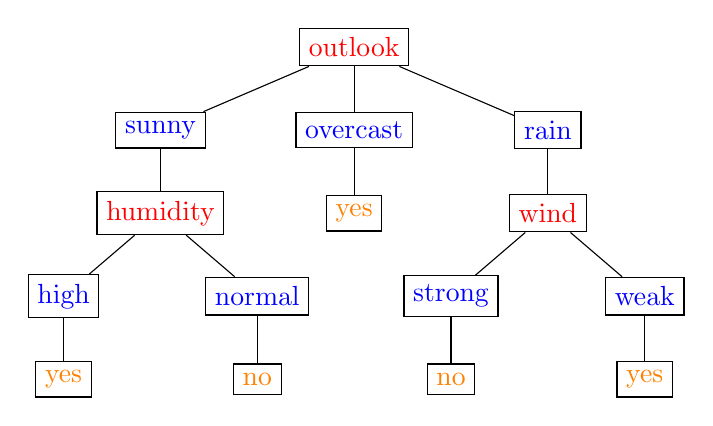
\begin{tikzpicture}[nodes={draw}, -, sibling distance=70pt, level
      distance=30pt]  
      \node{\color{red} outlook}
      child { node {\color{blue} sunny}
        child{ node {\color{red} humidity}
          child{ node {\color{blue} high}
            child{ node {\color{orange} yes}}}
          child{ node {\color{blue} normal}
            child{ node {\color{orange} no}}}}}
      child { node {\color{blue} overcast}
        child { node {\color{orange} yes}}}
      child { node {\color{blue} rain}
        child{ node {\color{red} wind}
          child{ node {\color{blue} strong}
            child{ node {\color{orange} no}}}
          child{ node {\color{blue} weak}
            child{ node {\color{orange} yes}}}}};
    \end{tikzpicture}
  \caption{Esempio di albero decisionale}
  \label{dt}
\end{figure}

Avanzando nell'albero cerchiamo una risposta (che ci deve essere).\\
La flessibilità nella costruzione dell'albero sta nel scegliere gli attributi e
i valori di ognuno. Con l'algoritmo \textbf{ID3} si costruiscono alberi
decisionali in base alle istanze che ricevo cosi da avere un albero coerente con le
istanze ricevute.\\
Formule booleane possono essere rappresentate in un albero decisionale (figura
\ref{dt2} e figura \ref{dt3}), costruendo un albero che sia \textit{yes}
solo nei casi la formula booleana 
sia vera.
\begin{figure}[H]
  \centering
  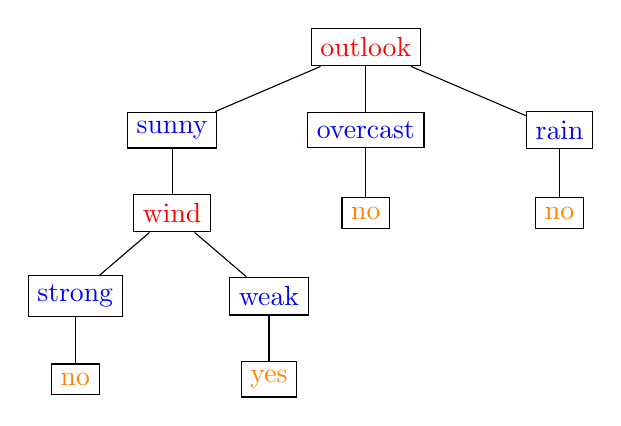
\begin{tikzpicture}[nodes={draw}, -, sibling distance=70pt, level
    distance=30pt]  
    \node{\color{red} outlook}
    child { node {\color{blue} sunny}
      child{ node {\color{red} wind}
        child{ node {\color{blue} strong}
          child{ node {\color{orange} no}}}
        child{ node {\color{blue} weak}
          child{ node {\color{orange} yes}}}}}
    child { node {\color{blue} overcast}
      child { node {\color{orange} no}}}
    child { node {\color{blue} rain}
      child{ node {\color{orange} no}}};
  \end{tikzpicture}
  \caption{Esempio di albero decisionale per la formula $(Outlook=Sunny)\land
    (Wind=Weak)$} 
  \label{dt2}
\end{figure}
\begin{figure}[H]
  \centering
  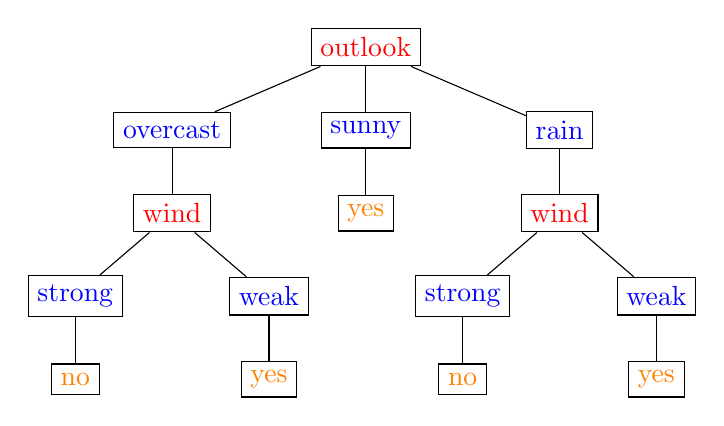
\begin{tikzpicture}[nodes={draw}, -, sibling distance=70pt, level
    distance=30pt]  
    \node{\color{red} outlook}
    child { node {\color{blue} overcast}
      child{ node {\color{red} wind}
        child{ node {\color{blue} strong}
          child{ node {\color{orange} no}}}
        child{ node {\color{blue} weak}
          child{ node {\color{orange} yes}}}}}
    child { node {\color{blue} sunny}
      child{ node {\color{orange} yes}}}
    child { node {\color{blue} rain}
      child{ node {\color{red} wind}
        child{ node {\color{blue} strong}
          child{ node {\color{orange} no}}}
        child{ node {\color{blue} weak}
          child{ node {\color{orange} yes}}}}};
  \end{tikzpicture}
  \caption{Esempio di albero decisionale  per la formula $(Outlook=Sunny)\lor
    (Wind=Weak)$}
  \label{dt3}
\end{figure}
Notiamo a questo punto come l'albero decisionale in figura \ref{dt} è la
rappresentazione di:
\[(Outlook=Sunny\,\land\, Humidity=Normal)\]
\[\lor(Outlook=Overcast)\]
\[\lor(Outlook=Rain \land Wind=Weak) \] 
Possiamo dire che gli alberi decisionali descrivono tutte le funzioni
booleane. Avendo $n$ funzioni booleane avremo un numero distinto di tabelle di
verità (e quindi di alberi decisionali), ciascuna con $2^n$ righe, pari a
$2^{2^{n}}$.\\
Riassumiamo alcune caratteristiche degli alberi decisionali:
\begin{itemize}
  \item Abbiamo attributi con valori discreti.
  \item Abbiamo un target di uscita discreto, per cui le foglie hanno valori precisi.
  \item Posso costruire ipotesi anche con disgiunzioni.
  \item Può esserci ``rumore'' nel training dei dati.
  \item Possono esserci attributi di cui non ho informazioni.
\end{itemize}
\subsubsection{Esercitazione sugli alberi decisionali}
Partiamo con un esercizio con find-S per coglierne le problematiche.
\begin{esercizio}
  Siano dati due attributi $A=\{1,2,3\}$ e $B=\{1,2\}$. Diciamo che $H$ è un
  congiunzione di $and$ tra i valori degli attributi e delle istanze.\\
  Il concetto target è:
  \[c:=((A=1\lor A=2), B=1)\]
  Find-S può trovare $c$ in $H$?\\
  Prendo un training set contenente $\langle x_1=(1,1), 1\rangle$ e
  $x_2=\langle(2,1),1\rangle$. Seguendo find-S 
  avremo la seguente traccia dell'algoritmo:
  \begin{table}[H]
    \centering
    \begin{tabular}{c|c}
      A & B\\
      \hline
      $\emptyset$ & $\emptyset$\\
      1 & 1 \\
      ? & 1
    \end{tabular}
  \end{table}
  Si arriva quindi a:
  \[S=\langle ?,1\rangle\]
  Ma questa generalizzazione mi farebbe accettare $A=3$, cosa non prevista da
  $c$.\\
  Non posso quindi usare find-S in questo caso.
\end{esercizio}
Ricordiamo che un albero decisionale è formato da:
\begin{itemize}
  \item \textbf{Nodes (\textit{nodi})}: etichettati da i vari attributi.
  \item \textbf{Branches \textit{rami}}: etichettati con i possibili valori
  dell'attributo che etichetta il nodo sorgente del ramo.
  \item \textbf{Leef nodes (\textit{foglie})}: etichettati con gli outcome della
  previsione.
\end{itemize}
Un percorso dalla radice fino alla foglia mi rappresenta una congiunzione di
attributi mentre l'albero in se è una disgiunzione di congiunzioni, una
per ogni percorso radice-foglia. Un albero formalizza la congiunzione di
vincoli su attributi ma può estendere il linguaggio per accettare delle disgiunzioni di vincoli su questi ultimi.\\
Usando funzioni booleane \footnote{un attributo può avere valore $\top,\,\,\,T$ o
$\bot,\,\,\,F$} posso convertire tabelle di verità in alberi decisionali, avendo ogni percorso dalla radice ad una foglia che rappresenta una
\textbf{regola}, e l'intero albero rappresenta la congiunzione di tutte le
regole. Le foglie quindi sono gli assegnamenti di verità della tabella.\\ 
Posso avere alberi diversi a seconda della scelta del nodo radice.\\
\begin{esempio}
  Vediamo i due alberi per la funzione booleana $\lor$.\\
  Abbiamo la tabella di verità:
  \begin{table}[H]
    \centering
    \begin{tabular}{c|c|c}
      $A$ & $B$ & $B\lor B$\\
      \hline
      $T$ & $T$ & $T$\\
      $T$ & $F$ & $T$\\
      $F$ & $T$ & $T$\\
      $F$ & $F$ & $F$
    \end{tabular}
  \end{table}
  rappresentata dai due alberi:
  \begin{figure}[H]
    \centering
    \includegraphics[scale = 0.9]{img/dt1.pdf}
  \end{figure}
\end{esempio}
Essendo sempre nel concept learning, nel caso di funzioni booleane, anche il
target è booleano.
\begin{teorema}
  Con un albero decisionale posso rappresentare tutte le
  funzioni booleane
\end{teorema}
\begin{proof}
  Prendiamo una qualsiasi funzione booleana e la traduciamo in tabella di
  verità.\\
  A partire dalla tabella costruisco l'albero decisionale dove ogni percorso
  radice-foglia è un esempio, ovvero una riga, della tabella di verità.\\
  Dato che ogni funzione booleana può essere rappresentata con una tabella di
  verità posso costruire un albero decisionale per qualsiasi funzione booleana.
\end{proof}
Seppur il metodo appena descritto dimostri il teorema, non è sempre
efficiente, per via del fatto che necessita di memorizzare sempre tutto.
\begin{teorema}
  Avendo una funzione booleana con $n$ attributi allora posso costruire una
  tabella di verità con $2^n$ righe. Potenzialmente posso costruire 
  $2^{2^n}$ alberi decisionali differenti aventi lo stesso significato.
\end{teorema}
Vediamo quindi un algoritmo generale per la costruzione dell'albero:
\begin{enumerate}
  \item Si inizia con un albero vuoto.
  \item Scelgo un attributo opportuno da impostare come nodo radice per fare lo \textit{split} dei dati.
  \item Per ogni \textit{split} dell'albero:
  \begin{itemize}
    \item Se non ho altro da fare, calcolo la la predizione con l'ultimo nodo foglia.
    \item Altrimenti si torna allo step 2 e si procede con un altro \textit{split}.
    \textit{split}
  \end{itemize}
\end{enumerate}
Bisognerà capire:
\begin{itemize}
  \item Come fare in modo ottimizzato lo `\textit{split}
  \item Quando fermare la costruzione dell'albero.
\end{itemize}
\begin{esempio}
  Prendiamo il solito esempio giocattolo di quando andare a fare sport in base
  al clima.\\
  In base al valore di \textit{outlook} ottengo tre tabelle, le quali si basano sul valore del campo \textit{overcast}, mantenendo comunque il target sul campo $play$ (nell'immagine il terzo arco è etichettato con
  $rainy$ e non con $text$):
  \begin{figure}[H]
    \centering
    \includegraphics[scale = 0.9]{img/dt2.pdf}
  \end{figure}
  \begin{table}[H]
    \centering
    \begin{tabular}{c|c|c|c|c}
      outlook & temp & humidity & windy & play\\
      \hline
      overcast & H & H & $\bot$ & \color{darkgreen}{yes}\\
      overcast & C & N & $\top$ & \color{darkgreen}{yes}\\
      overcast & M & H & $\top$ & \color{darkgreen}{yes}\\
      overcast & H & N & $\bot$ & \color{darkgreen}{yes}
    \end{tabular}
    \caption{Tabella A}
  \end{table}
  \begin{table}[H]
    \centering
    \begin{tabular}{c|c|c|c|c}
      outlook & temp & humidity & windy & play\\
      \hline
      sunny & H & H & $\bot$ & \color{red}{no}\\
      sunny & H & H & $\top$ & \color{red}{no}\\
      sunny & M & H & $\bot$ & \color{red}{no}\\
      sunny & C & N & $\bot$ & \color{darkgreen}{yes}\\
      sunny & M & N & $\top$ & \color{darkgreen}{yes}
    \end{tabular}
    \caption{Tabella B}
  \end{table}
  \begin{table}[H]
    \centering
    \begin{tabular}{c|c|c|c|c}
      outlook & temp & humidity & windy & play\\
      \hline
      rainy & M & H & $\bot$ & \color{darkgreen}{yes}\\
      rainy & C & N & $\bot$ & \color{darkgreen}{yes}\\
      rainy & C & N & $\top$ & \color{red}{no}\\
      rainy & M & N & $\bot$ & \color{darkgreen}{yes}\\
      rainy & M & H & $\top$ & \color{red}{no}
    \end{tabular}
    \caption{Tabella C}
  \end{table}
 
  Vediamo un secondo i valori del target nei vari casi:
  \begin{itemize}
    \item Nel caso di \textit{overcast} ho 4 \textit{yes} e 0 \textit{no}
    \item Nel caso di \textit{sunny} ho 2 \textit{yes} e 3 \textit{no}
    \item Nel caso di \textit{rainy} ho 3 \textit{yes} e 2 \textit{no}
  \end{itemize}
  Posso quindi usare una \textbf{funzione di costo} per fissare quando una
  distribuzione è omogenea (come nel caso di \textit{overcast}) e quando no (gli
  altri due casi). Lo \textit{split} infatti andrebbe fatto in base ai valori
  del target: più sono omogenei e meglio è; in quanto nel momento in cui si
  presenta un nuovo test per la classificazione con \textit{outlook} pari a
  \textit{overcast} saprò già cosa fare (in quanto nello storico delle
  esperienze ho sempre avuto \textit{yes}). Le altre due situazioni sono
  ambigue e, in quei due casi, devo procedere con la costruzione
  dell'albero per ottenere informazioni cercando di rimuovere l'incertezza.  
\end{esempio}
La \textbf{funzione costo} è alla base della strategia della costruzione
dell'albero.\\
Una strategia può essere quella ``a maggioranza'', prendendo l'attributo che con
i suoi valori ha meno disomogeneità. Per farlo calcolo la differenza tra $yes$ e
$no$ di ogni valore per un certo attributo, sommandone i risultati. Scelgo
l'attributo con più omogeneità (ovvero quello con la somma piu bassa), che ha una
distribuzione più pulita dei risultati. Se ho valori con solo
$yes$ o solo $no$ sommo 0.
\begin{esempio}
  Prendendo le tre tabelle sopra, per \textit{outlook} avrei:
  \[0+1+1=2\]
  Se avessi avuto un attributo con:
  \begin{itemize}
    \item Primo valore: 1 \textit{yes} e 1 \textit{no}
    \item Secondo valore: 2 \textit{yes} e 0 \textit{no}
    \item Terzo valore: 0 \textit{yes} e 4 \textit{no}
    \item Quarto valore: 2 \textit{yes} e 4 \textit{no}
    \item Quinto valore: 2 \textit{yes} e 2 \textit{no} 
  \end{itemize}
  avrei avuto:
  \[1+0+0+2+2=5\]
\end{esempio}
Gli alberi di decisione possono essere utilizzati anche nel continuo, per
attributi numerici.
\begin{esempio}
  Prendiamo le istanze definite da due attributi, $x$ e $y$ e costruisco un
  albero di decisione che definisce in quali aree del piano ho $-$ e quali ho
  $+$.
  \newpage
  Si ha il seguente piano (\textbf{sull'asse delle $y$ il primo valore a partire
  dall'origine è un 5 non un 7}): 
  \begin{figure}[H]
    \centering
    \includegraphics[scale = 0.8]{img/dt3.pdf}
  \end{figure}
  E si ottiene, per esempio, il seguente albero decisionale:
  \begin{figure}[H]
    \centering
    \includegraphics[scale = 0.9]{img/dt4.pdf}
  \end{figure}
  Dove a ciascun nodo è associata una condizione e agli archi il fatto che sia
  verificata o meno.\\
  Si nota come non si hanno tutte le condizioni, infatti, per esempio, con $x>3$
  mi basta $y>7$ per trovare il $+$ e $y<7$ per il $-$ (non dovendo andare
  specificatamente a guardare anche $y<5$ o $y>5$).\\
  \textbf{Quello disegnato è solo uno dei possibili alberi.}
\end{esempio}
\subsection{Algoritmo ID3}
Vista la difficoltà di scegliere l'albero si ha l'idea di scegliere un piccolo
albero di partenza (o più piccoli) e ricorsivamente l'attributo più
significativo (sia nei nodi rossi intermedi che nelle foglie) come radice per il
sotto-albero. Si fanno quindi crescere in modo 
coerente gli alberi piccoli scelti in partenza. Si punta ad arrivare ad un
albero valido per tutti gli esempi ricevuti e anche per quelli non visti.\\
Iniziamo a vedere l'algoritmo anche se saranno necessarie molte specifiche:
\begin{algorithm}[H]
  \begin{algorithmic}
    \Function{ID3}{}
    \State $A \gets$ \textit{il ``miglior'' attributo di decisione per il
    prossimo nodo}
    \State \textit{assegno A come attributo di decisione per il nodo, che sarà
    rosso}
    \For {\textit{ogni valore dell'attributo A}}
    \State \textit{creo un discendente}
    \EndFor
    \State \textit{ordina gli esempi di training alla foglia}
    \State \textit{in base al valore dell'attributo del branch}
    \If {\textit{ho classificato tutti gli esempi di training}}
    \State \textit{mi fermo}
    \Else
    \State \textit{itero sulle foglie appena create}
    \EndIf
    \EndFunction
  \end{algorithmic}
  \caption{Algoritmo ID3 (Iterative Dichotomiser 3)}
\end{algorithm}
Il \textbf{bias induttivo} su ID3 è che preferisce alberi piccoli.\\
Bisogna in primis capire cosa si intende come \textbf{attributo migliore}. Per
farlo introduciamo la seguente notazione:
\[[esempi\,\,\,positivi+,\,\,esempi\,\,\,negativi-]\]
entrambi rappresentati con un valore intero. Gli esempi positivi sono gli esempi
che già mi hanno restituito \textit{yes} mentre quelli negativi sono quelli che mi hanno restituito \textit{no}.
Vediamo quanto detto:

\begin{figure}[H]
  \centering
  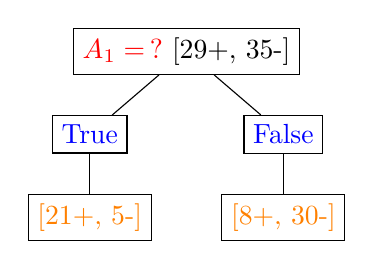
\begin{tikzpicture}[nodes={draw}, -, sibling distance=70pt, level
    distance=30pt]  
    \node{\color{red} $A_1=\,?$ \color{black} [29+, 35-]}
    child { node {\color{blue} True}
      child{ node {\color{orange} [21+, 5-]}}}
    child { node {\color{blue} False}
      child{ node {\color{orange} [8+, 30-]}}};
  \end{tikzpicture}
\end{figure}

Se siamo nella situazione in cui dobbiamo confrontare l'attributo sopra con un
altro, per esempio:
\begin{figure}[H]
  \centering
  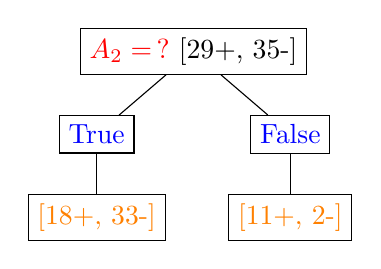
\begin{tikzpicture}[nodes={draw}, -, sibling distance=70pt, level
    distance=30pt]  
    \node{\color{red} $A_2=\,?$ \color{black} [29+, 35-]}
    child { node {\color{blue} True}
      child{ node {\color{orange} [18+, 33-]}}}
    child { node {\color{blue} False}
      child{ node {\color{orange} [11+, 2-]}}};
  \end{tikzpicture}
\end{figure}
Entrambe le foglie del primo attributi ci parlano di valori sbilanciati (tra
esempi positivi e negativi), a differenza delle due del secondo attributo, dove
sono una sbilanciata e una no. Per ora stabiliamo ad occhio lo sbilanciamento.\\
Il criterio di scelta ci porta a preferire lo sbilanciamento, verso un ideale
``tutti positivi'' o ``tutti negativi''. Quindi se un attributo ha divisioni
sbilanciate è da ritenersi migliore.\\ 
Per essere ancora più precisi bisogna richiamare la matematica
dell'\textbf{entropia}.
\begin{definizione}
  Dato un training set $S$ con valori $v_i,\,\,i=1\ldots n$. l'entropia di un
  insieme di bit misura più o meno la sua quantità di informazione. La formula per il calcolo dell'entropia su un set $S$ è:
  \[I(P(v_1),\ldots,P(v_n))=\sum_{i=1}-P(v_i)\log_2P(v_i)\]
  Dove $I(x)$ indica il valore dell'entropia su $x$ e $P(y)$ sta per la
  probabilità legata ad un valore $y$.  \\
  Nel caso booleano le istanze presenti in un certo insieme $S$ sono associate
  ad un'etichetta, e vengono conteggiate. Nella variabile $p$ conto i valori di $S$ con
  etichetta positiva e con $n$ negativa. Ottengo
  quindi in modo esplicito la sommatoria:
  \[I\left(\frac{p}{p+n},\frac{n}{p+n}\right)=-\frac{p}{p+n}\log_2\frac{p}{p+n}
    -\frac{n}{p+n}\log_2\frac{n}{p+n}\]  
  Se inoltre diciamo che $p_+$ è la proporzione di esempi positivi e $p_-$ di
  quelli negativi (saranno quindi tra 0 e 1) possiamo misurare
  l'\textbf{impurità} di $S$ con l'entropia: 
  \[Entropy(S)=-p_+\log_2 p_+-p_-\log_2 p_-\]
  Avrò un'alta entropia se positivi e negativi sono ``metà e metà''
\end{definizione}
Parliamo quindi di \textbf{information gain} $IG$ che viene calcolato su ogni
attributo $A$ e su $S$:
\[IG(S,A)=I\left(\frac{p}{p+n},\frac{n}{p+n}\right)-remainder(A)\]
dove:
\[remainder(A)=\sum_{i=1}^v \frac{p_i+n_i}{p+n}
  I\left(\frac{p_i}{p_i+n_i},\frac{n_i}{p_i+n_i}\right)\]
l'information gain è la riduzione aspettata nell'entropia per ordinare
$S$ sull'attributo $A$. Si sceglie l'attributo con il maggiore IG.\\
Possiamo riscrivere il conto come:
\[IG(S,A)=Entropy(S)-\sum_{v\in values(A)}\frac{|S_v|}{|S|}Entropy(S_v)\]
\begin{esempio}
  Vediamo l'esempio di calcolo di entropia di $A_1$ con [29+,35-]:
  \[Entropy([29+,35-])=
    -\frac{29}{64}\log_2\frac{29}{64}-\frac{35}{64}\log_2\frac{35}{64}=0.99\]
  Calcolo anche l'information gain di $A_1$, sapendo che
  $Entropy([21+,5-])=0.71$ e $Entropy([8+,30-])=0.74$,
  e quindi:
  \[IG(S,A_1)=0.99-\frac{26}{64}\cdot 0.71-\frac{38}{64}\cdot 0.74=0.27\]
  ugualmente calcolo $IG(S,A_2)=0.12$. \\
  Quindi so che devo scegliere $A_1$ in quanto $0.27 > 0.12$
\end{esempio}
Facciamo qualche osservazione finale sull'\textbf{algoritmo ID3}:
\begin{itemize}
  \item Lo spazio delle ipotesi è completo e sicuramente contiene il target.
  \item Ho in output una singola ipotesi.
  \item Non si ha backtracking sugli attributi selezionati, si procede con una
  ricerca greedy, trovando scelte buone localmente ma non ottime.
  \item Fa scelte basate su una ricerca statistica, facendo sparire incertezze
  sui dati.
  \item Il bias non è sulla classe iniziale, essendo lo spazio delle ipotesi
  completo, ma sulla scelta di solo alcune funzioni, preferendo alberi corti (e
  più semplici) e posizionando attributi ad alto information gain vicino alla
  radice. Il bias è quindi sulla preferenza di alcune ipotesi. Si usa il
  criterio euristico di \textit{rasoio di Occam}.
  \item $H$ è l'insieme potenza delle istanze $X$.
\end{itemize}
Viene introdotto però l'\textbf{overfitting}.
\begin{definizione}
  \textit{Definizione tratta da wikipedia.}\\
  Definiamo formalmente l'\textbf{overfitting} come l'adattamento eccessivo,
  ovvero quando 
  un un modello statistico molto complesso si adatta al campione perché ha un
  numero eccessivo di parametri rispetto al numero di osservazioni. SI ha
  quindi che un modello assurdo e sbagliato può adattarsi perfettamente se è
  abbastanza complesso rispetto alla quantità di dati disponibili.\\
  Nel machine learning se il learner viene addestrato troppo a lungo il modello
  potrebbe adattarsi a caratteristiche che sono specifiche solo del training
  set, ma che non hanno riscontro nel resto dei casi quindi le prestazioni sui
  dati non visionati saranno drasticamente peggiori.\\
  L'opposto è l'\textbf{underfitting}.
\end{definizione}

Se misuro l'errore di una ipotesi
$h$ sul training set ($error_{traini}(h)$) e poi misuro l'errore di quella
ipotesi sull'intero set delle possibili istanze
$D$ ($error_D(h)$) ho che l'ipotesi $h$ va in \textbf{overfit} sul quel data set
se:
\[error_{traini}(h) < error_{traini}(h') \,\,\land
  \,\,error_D(h)>error_D(h')\]
quindi se presa un'altra ipotesi questa è migliore della prima e ha un errore
sull'intera distribuzione delle ipotesi inferiore vado in \textit{overfit}. Il
problema è che non posso sapere se esiste tale $h'$. Per evitare il problema uso
sempre il rasoio di Occam scegliendo ipotesi semplici ed evitando di far
crescere l'albero quando lo ``split'' non è statisticamente significativo. Un
altro modo è quello di togliere pezzi, all'albero, che toccano poche istanze o
pure calcolare una \textit{misura di complessità dell'albero}, minimizzando la
grandezza dell'albero e gli errori del \textit{training set}, usando il
\textbf{Minimum Description Length (\textit{MDL})}.\\
In ID3 quindi posso scegliere sia in base all'\textit{information gain} massimo
o all'\textit{entropia} minima tra gli attributi.
\subsubsection{Esercitazione su ID3}
Quando parliamo di \textit{entropia} stiamo volgendo un esperimento
concettuale. Prima dell'esperimento si ha una certa incertezza su un certo
eventi, che sparisce, con sorpresa, una volta eseguito l'esperimento se l'evento
accade. D'altro canto qualora accade un evento atteso siamo meno sorpresi del
fatto. Nel primo caso però si ritiene di ottenere molta informazione, nel
secondo caso poca. Come se ponessimo in una vasca quattro palline rosse, non
sarei stupito di estrarne una rossa, essendo quello che mi aspetto. D'altro
canto se ne aggiungo quattro verdi l'estrazione sarà inattesa e quindi più
interessante.\\ 
Si cerca un modo di quantificare questa ``sorpresa''. Riprendendo l'esempio
della palline posso dire che nel primo caso (solo rosse) ho \textbf{bassa
  entropia} e nel secondo caso (palline miste) \textbf{alta entropia}. Un caso
intermedio sarebbe a \textbf{media entropia}.\\
Quindi, detta $P(x)$ la probabilità che avvenga un evento $x$ e con $I(p)$
l'informazione che ottengo dopo che l'evento si è verificato:
\begin{itemize}
  \item $P(x)=1\to I(p)=0$
  \item $P(x)=0\to I(p)=\infty$
\end{itemize}
L'informazione $I(p)$ e quindi una quantità non negativa:
\[I(p)\geq 0\]
Definiamo quindi l'informazione, detta anche \textit{self-information}, per un
evento $E$: 
\[I(E)=-\log_2(P(E))\]
Inoltre ho che è additiva se gli eventi sono indipendenti, ovvero:
\[I(p_1,p_2)=I(p_1)+I(p_2)\]
Bisogna però estendere l'informazione a tutte le possibili distribuzioni di
tutti i possibili esiti che ho in un esperimento concettuale.\\
Passiamo quindi alle definizioni matematiche per l'\textbf{entropia}:
\begin{itemize}
  \item $X\sim P_X$, presa una certa variabile $X$ dell'esperimento con una
  certa funzione di probabilità associata $P_X$
  \item $Val(X)=\{x_1,\ldots,x_n\}$, ovvero il range di valori della variabile
  $X$
  \item $p_i=P_X(x_i)$, probabilità per quel valore della variabile $X$
  \item $g:\mathbb{R}\to\mathbb{R}$ una funzione arbitraria tale per cui $g(X)$
  è una variabile causale. Si definisce l'aspettativa di $G(X)$ su $P$ come:
  \[E_P[g(X)]=\sum_{x\in Val(X)} g(x)\cdot P_X(x)\]
\end{itemize}
Giungendo quindi alla formula dell'\textbf{entropia} di una variabile:
\[H[X]=-\sum_{i=1}^n p_i\cdot\log_2 p_i=E_P[\log_2(p)]\]
Quindi:
\begin{definizione}
  L'\textbf{entropia}, definita da Claude Shannon (e quindi spesso chiamata
  \textbf{entropia di Shannon}), è l'informazione media associata ad
  una distribuzione di probabilità.
\end{definizione}
Vediamo un esempio:
\begin{esempio}
  Suppongo di lanciare una moneta, si ha:
  \[P(testa)=P(croce)=\frac{1}{2}\]
  Definiamo che testa è specificata da $X=0$ e croce da $X=1$.\\
  Calcoliamo quindi:
  \[H(p)=-p(0)\cdot \log_2 p(0)-p(1)\cdot\log_2
    p(1)=-2\cdot(\frac{1}{2}\cdot\log_2\frac{1}{2})=1\] 
  Una moneta ``onesta'' ha quindi entropia pari a 1 (avendo due probabili esiti
  equiprobabili non ho certezza del risultato).\\
  Ipotizziamo di avere una moneta magica che cade solo sulla testa (quindi
  $P(0)=1$ e $P(1)=0$:
  \[H(p)=-p(0)\cdot \log_2 p(0)-p(1)\cdot\log_2 p(1)=-\log_2 (1)=0\]
  Una moneta ``non onesta'' ha quindi entropia pari a 0 (ho infatti certezza del
  risultato).
\end{esempio}
\begin{esempio}
  Considero il seguente training set, con 4 esempi e target $T$:
  \begin{table}[H]
    \centering
    \begin{tabular}{c|c|c|c|c|c}
      example & A & B & C & D & T\\
      \hline
      $x_1$ & 0 & 0 & 1 & 1 & \color{darkgreen}{1}\\
      $x_2$ & 0 & 1 & 1 & 1 & \color{darkgreen}{1}\\
      $x_3$ & 0 & 1 & 0 & 0 & \color{red}{0}\\
      $x_4$ & 0 & 1 & 0 & 1 & \color{darkgreen}{1}\\
    \end{tabular}
  \end{table}
  Si ha quindi la seguente distribuzione di probabilità relativa al target
  (avendo un \textit{no} e tre \textit{yes}):
  \[P_T=\left[\frac{1}{4},\frac{3}{4}\right]\]
  e quindi posso calcolare l'entropia della tabella:
  \[H(P_T)=-P_T(0)\cdot \log_2 P_T(0)-P_T(1)\cdot\log_2
    P_T(1)=-\frac{1}{4}\cdot\log_2\frac{1}{4}-\frac{3}{4}\cdot\log_2
    \frac{3}{4}= 0.81\]
  La tabella può essere vista come un risultato di un esperimento concettuale.
\end{esempio}
\begin{definizione}
  Definiamo l'\textbf{entropia di una distribuzione condizionale}. Presa $X$
  come una variabile discreta arbitraria con valori $\{x_1,\ldots,x_n\}$, che
  hanno ciascuno probabilità $P_X(x_i)$ ho che, per la distribuzione
  condizionale:
  \[P{Y|X=x_i}(y_j)=P_{Y|X}(y_j|x_i)\]
  Ovvero la distribuzione dei valori della variabile $Y$ dato $X=x_i$.\\
  Quindi voglio sapere la probabilità di $Y$ condizionata da un esperimento
  precedente su $X$.\\
  Per l'entropia ho:
  \[H_{Y|X=x_i}=-\sum_{j=1}^m P_{Y|X}(y_j|x_i)\cdot \log_2 P_{Y|X}(y_j|x_i)\]
  quindi è la solita formula ma con la probabilità condizionale.
\end{definizione}
\begin{definizione}
  Definiamo \textbf{entropia condizionale} come il valore medio, ovvero il
  valore atteso, dell'entropia di $p_{Y|X=x_i}$ per ciascun valore di $X$ che
  condiziona $Y$, ovvero:
  \[H_{Y|X}=\sum_{i=1}^n P_X(x_i)H_{Y|X=x_i}\]
  ottenendo l'\textbf{entropia condizionale}:
  \[H[Y|X]=\sum P(x)\cdot H(Y|X=x)\]
\end{definizione}
\begin{esercizio}
  Considero il seguente training set, con 4 esempi e target $T$:
  \begin{table}[H]
    \centering
    \begin{tabular}{c|c|c|c|c|c}
      example & A & B & C & D & T\\
      \hline
      $x_1$ & 0 & 0 & 1 & 1 & \color{darkgreen}{1}\\
      $x_2$ & 0 & 1 & 1 & 1 & \color{darkgreen}{1}\\
      $x_3$ & 0 & 1 & 0 & 0 & \color{red}{0}\\
      $x_4$ & 0 & 1 & 0 & 1 & \color{darkgreen}{1}\\
    \end{tabular}
  \end{table}
  Abbiamo già calcolato l'entropia associabile al valore target $H[P_T]=0.81$.\\
  Passiamo ora all'uso di ID3 per la costruzione dell'albero.\\
  Dobbiamo cercare gli split corretti tramite information gain, usando
  l'entropia condizionale.\\
  Partiamo con il primo attributo: $A$. Si ha che $P_A(0)=1$ e $P_A(1)=0$,
  quindi:
  \[H[T|A=0]=-p_{T|A}(0|0)\cdot \log_2(p_{T|A}(0|0))-p_{T|A}(1|0)\cdot
    \log_2(p_{T|A}(1|0))=\]
  \[-\frac{1}{4}\cdot\log_2\frac{1}{4}-
    \frac{3}{4}\cdot\log_2\frac{3}{4}=0.81\]
  (Risultato pari a quello dell'intero training set in quanto $A$ è sempre 0)\\
  Non devo calcolare $H[T|A=1]$ in quanto $A$ non è mai pari ad 1.\\
  Inoltre si ha:
  \[H[T|A]=P_A(0)\cdot H[T|A=0]+P_A(1)\cdot H[T|A=1]=1\cdot 0.81=0.81\]
  Posso quindi calcolare l'\textit{information gain}:
  \[IG[T;A]=H[T]-H[T|A]=0.81-0.81=0\]
  Quindi per $A$ ho la seguente distribuzione del target (avendo nel target 3
  esempi positivi e uno negativo e $A$ sempre con valore 0):
  \begin{figure}[H]
    \centering
    \includegraphics[scale = 0.9]{img/id1.pdf}
  \end{figure}
 \textbf{\textit{Ricordiamo che ID3 sceglie per lo splitting l'attributo che
     rende massimo l'information gain.}}\\
  Passo quindi all'attributo $B$. Si ha che $P_B(0)=\frac{1}{4}$ e
  $P_B(1)=\frac{3}{4}$, quindi:
  \[H[T|B=0]=-p_{T|B}(0|0)\cdot \log_2(p_{T|B}(0|0))-p_{T|B}(1|0)\cdot
    \log_2(p_{T|B}(1|0))=\]
  \[-0\cdot \log_2 0-1\cdot \log_2 1=0\]
  e:
  \[H[T|B=1]=-p_{T|B}(0|1)\cdot \log_2(p_{T|B}(0|1))-p_{T|B}(1|1)\cdot
    \log_2(p_{T|B}(1|1))=\]
  \[-\frac{1}{3}\cdot\log_2\frac{1}{3}-
    \frac{2}{3}\cdot\log_2\frac{2}{3}=0.91\]
  (ho quindi una partizione migliore con $B=0$)\\
  Inoltre si ha:
  \[H[T|B]=P_B(0)\cdot H[T|B=0]+P_B(1)\cdot H[T|B=1]=\frac{1}{4}\cdot
    0+\frac{3}{4}\cdot 0.91=0.68\]
  Posso quindi calcolare l'\textit{information gain}:
  \[IG[T;B]=H[T]-H[T|B]=0.81-0.68=0.13\]
  Quindi per $B$ ho:
  \begin{figure}[H]
    \centering
    \includegraphics[scale = 0.9]{img/id2.pdf}
  \end{figure}
  Ho quindi un partizionamento più interessante.\\
  Passo quindi all'attributo $C$. Si ha che $P_C(0)=\frac{1}{2}$ e
  $P_C(1)=\frac{1}{2}$, quindi:
  \[H[T|C=0]=-p_{T|C}(0|0)\cdot \log_2(p_{T|C}(0|0))-p_{T|C}(1|0)\cdot
    \log_2(p_{T|C}(1|0))=\]
  \[-\frac{1}{2}\cdot \log_2 \frac{1}{2}-\frac{1}{2}\cdot \log_2 \frac{1}{2}=1\]
  e:
  \[H[T|C=1]=-p_{T|C}(0|1)\cdot \log_2(p_{T|C}(0|1))-p_{T|C}(1|1)\cdot
    \log_2(p_{T|C}(1|1))=\]
  \[-0\cdot \log_2 0-1\cdot \log_2 1=0\]
  Inoltre si ha:
  \[H[T|C]=P_C(0)\cdot H[T|C=0]+P_C(1)\cdot H[T|C=1]=\frac{1}{2}\cdot
    1+\frac{1}{2}\cdot 0=\frac{1}{2}\]
  Posso quindi calcolare l'\textit{information gain}:
  \[IG[T;C]=H[T]-H[T|C]=0.81-\frac{1}{2}=0.31\]
  Quindi per $C$ ho:
  \begin{figure}[H]
    \centering
    \includegraphics[scale = 0.9]{img/id3.pdf}
  \end{figure}
  $C$ migliora ancora il partizionamento.\\
  Passo quindi all'attributo $D$. Si ha che $P_D(0)=\frac{1}{4}$ e
  $P_D(1)=\frac{3}{4}$, quindi:
  \[H[T|D=0]=-p_{T|D}(0|0)\cdot \log_2(p_{T|D}(0|0))-p_{T|D}(1|0)\cdot
    \log_2(p_{T|D}(1|0))=\]
  \[-1\cdot \log_2 1-0\cdot \log_2 0=0\]
  e:
  \[H[T|D=1]=-p_{T|D}(0|1)\cdot \log_2(p_{T|D}(0|1))-p_{T|D}(1|1)\cdot
    \log_2(p_{T|D}(1|1))=\]
  \[-0\cdot \log_2 0-1\cdot \log_2 1=0\]
  Inoltre si ha:
  \[H[T|D]=P_D(0)\cdot H[T|D=0]+P_D(1)\cdot H[T|D=1]=\frac{1}{4}\cdot
    0+\frac{3}{4}\cdot 0=0\]
  Posso quindi calcolare l'\textit{information gain}:
  \[IG[T;D]=H[T]-H[T|D]=0.81-0=0.81\]
  Quindi per $D$ ho:
  \begin{figure}[H]
    \centering
    \includegraphics[scale = 0.9]{img/id4.pdf}
  \end{figure}
  $D$ rende quindi il massimo della ``purezza'' tra i valori di $D$ e quelli del
  target. Non ho incertezza nel partizionamento.\\
  Quindi, ricapitolando, ho i seguenti information gain:
  \begin{itemize}
    \item $IG[T;A]=0$
    \item $IG[T;B]=0.13$
    \item $IG[T;C]=0.31$
    \item $IG[T;D]=0.81$, \textbf{che è il valore massimo} e che rende minima la
    ``sorpresa''
  \end{itemize}
\end{esercizio}
\begin{esercizio}
  Considero il seguente training set, con 4 esempi e target $T$:
  \begin{table}[H]
    \centering
    \begin{tabular}{c|c|c|c|c|c}
      example & A & B & C & D & T\\
      \hline
      $x_1$ & 0 & 0 & 1 & $\ldots$ & \color{darkgreen}{1}\\
      $x_2$ & 0 & 1 & 1 & $\ldots$ & \color{darkgreen}{1}\\
      $x_3$ & 0 & 1 & 0 & $\ldots$ & \color{red}{0}\\
      $x_4$ & 0 & 1 & 0 & $\ldots$ & \color{darkgreen}{1}\\
    \end{tabular}
  \end{table}
  Bisogna riempire $D$ per rendere massimo l'information gain.
  \newpage
  Per farlo basta mettere gli stessi valori del target, in modo che sia
  l'attributo che meglio distribuisca i valori del target, ottenendo quindi lo
  stesso training set dell'esercizio precedente:
  \begin{table}[H]
    \centering
    \begin{tabular}{c|c|c|c|c|c}
      example & A & B & C & D & T\\
      \hline
      $x_1$ & 0 & 0 & 1 & 1 & \color{darkgreen}{1}\\
      $x_2$ & 0 & 1 & 1 & 1 & \color{darkgreen}{1}\\
      $x_3$ & 0 & 1 & 0 & 0 & \color{red}{0}\\
      $x_4$ & 0 & 1 & 0 & 1 & \color{darkgreen}{1}\\
    \end{tabular}
  \end{table}
  Un'alternativa è l'esatto opposto, in quanto otterrei la stessa
  ridistribuzione del target, rimuovendo ogni ``sorpresa'' ulteriore ma
  lasciando solo quella della tabella iniziale:
  \begin{table}[H]
    \centering
    \begin{tabular}{c|c|c|c|c|c}
      example & A & B & C & D & T\\
      \hline
      $x_1$ & 0 & 0 & 1 & 0 & \color{darkgreen}{1}\\
      $x_2$ & 0 & 1 & 1 & 0 & \color{darkgreen}{1}\\
      $x_3$ & 0 & 1 & 0 & 1 & \color{red}{0}\\
      $x_4$ & 0 & 1 & 0 & 0 & \color{darkgreen}{1}\\
    \end{tabular}
  \end{table}
\end{esercizio}
\begin{esercizio}
  Considero il seguente training set, con 4 esempi e target $T$:
  \begin{table}[H]
    \centering
    \begin{tabular}{c|c|c|c|c}
      example & $f_1$ & $f_2$ & $f_3$ & T\\
      \hline
      $x_1$ & 1 & 1 & 1 & \color{darkgreen}{1}\\
      $x_2$ & 0 & 1 & 1 & \color{red}{0}\\
      $x_3$ & 0 & 0 & 1 & \color{darkgreen}{1}\\
      $x_4$ & 0 & 0 & 0 & \color{red}{0}\\
    \end{tabular}
  \end{table}
  Vogliamo completare il seguente albero decisionale:
  \begin{figure}[H]
    \centering
    \includegraphics[scale = 0.75]{img/id5.pdf}
  \end{figure}
  Partendo da $f_1$ so che se arriva un nuovo esempio non potrò proseguire da
  $[0-,1+]$ in quanto so già che in quel caso avrei un'istanza positiva, valore
  minimo $0$.\\
  Quindi se $f_1=0$ vado a scegliere un nuovo attributo in quanto ancora non ho
  una distribuzione certa. Considero quindi le righe in cui $f_1=0$ e avanzo
  iterativamente studiando $f_2$ ed $f_3$. Studio quindi il sottoinsieme: 
  \begin{table}[H]
    \centering
    \begin{tabular}{c|c|c|c}
      example  & $f_2$ & $f_3$ & T\\
      \hline
      $x_2$ & 1 & 1 & \color{red}{0}\\
      $x_3$ & 0 & 1 & \color{darkgreen}{1}\\
      $x_4$ & 0 & 0 & \color{red}{0}\\
    \end{tabular}
  \end{table}
  e avanzo fino a che non finisco gli attributi (o arrivo in un punto in cui,
  come per il ramo 1 di $f_1$ non posso più continuare).\\
  Per questo nuovo sottoinsieme calcolo:
  \[P_T=\left[\frac{2}{3},\frac{1}{4}\right]\]
  e quindi posso calcolare l'entropia della tabella:
  \[H(P_T)=-P_T(0)\cdot \log_2 P_T(0)-P_T(1)\cdot\log_2
    P_T(1)=-\frac{2}{3}\cdot\log_2\frac{2}{3}-\frac{1}{3}\cdot\log_2
    \frac{1}{3}= 0.91\]
  Passo quindi all'attributo $f_2$. Si ha che $P_{f_2}(0)=\frac{2}{3}$ e
  $P_{f_2}(1)=\frac{1}{3}$, quindi:
  \[H[T|f_2=0]=-p_{T|f_2}(0|0)\cdot \log_2(p_{T|f_2}(0|0))-p_{T|f_2}(1|0)\cdot
    \log_2(p_{T|f_2}(1|0))=\]
  \[-\frac{1}{2}\cdot \log_2 \frac{1}{2}-\frac{1}{2}\cdot \log_2 \frac{1}{2}=1\]
  e:
  \[H[T|f_2=1]=-p_{T|f_2}(0|1)\cdot \log_2(p_{T|f_2}(0|1))-p_{T|f_2}(1|1)\cdot
    \log_2(p_{T|f_2}(1|1))=\]
  \[-0\cdot \log_2 0-1\cdot \log_2 1=0\]
  Inoltre si ha:
  \[H[T|f_2]=P_{f_2}(0)\cdot H[T|f_2=0]+P_{f_2}(1)\cdot
    H[T|f_2=1]=\frac{2}{3}\cdot 1+\frac{1}{3}\cdot 0=\frac{2}{3}\]
  Posso quindi calcolare l'\textit{information gain}:
  \[IG[T;f_2]=H[T]-H[T|f_2]=0.81-\frac{2}{3}=0.25\]
  
  Passo quindi all'attributo $f_3$. Si ha che $P_{f_3}(0)=\frac{1}{3}$ e
  $P_{f_3}(1)=\frac{2}{3}$, quindi:
  \[H[T|f_3=0]=-p_{T|f_3}(0|1)\cdot \log_2(p_{T|f_3}(0|1))-p_{T|f_3}(1|1)\cdot
    \log_2(p_{T|f_3}(1|1))=\]
  \[-1\cdot \log_2 1-0\cdot \log_2 0=0\]
  e:
  \[H[T|f_3=1]=-p_{T|f_3}(0|0)\cdot \log_2(p_{T|f_3}(0|0))-p_{T|f_3}(1|0)\cdot
    \log_2(p_{T|f_3}(1|0))=\]
  \[-\frac{1}{2}\cdot \log_2 \frac{1}{2}-\frac{1}{2}\cdot \log_2 \frac{1}{2}=1\]
  Inoltre si ha:
  \[H[T|f_3]=P_{f_3}(0)\cdot H[T|f_3=0]+P_{f_3}(1)\cdot
    H[T|f_3=1]=\frac{1}{3}\cdot 0+\frac{2}{3}\cdot 1=\frac{2}{3}\]
  Posso quindi calcolare l'\textit{information gain}:
  \[IG[T;f_3]=H[T]-H[T|f_3]=0.81-\frac{2}{3}=0.25\]
  Avendo $f_1$ e $f_2$ lo stesso $IG$ prendo il primo e quindi ho:
  \begin{figure}[H]
    \centering
    \includegraphics[scale = 0.9]{img/id6.pdf}
  \end{figure}
  Con $f_2$ che verrà attaccato al nodo $[2-,1+]$ ``uscente'' da $f_1$.\\
  A questo punto, come sopra, abbiamo che il nodo $[1-,0+]$ è foglia, avendo una
  distribuzione certa. Riduco quindi nuovamente il training set studiando solo
  gli esempi in cui $f_2$ vale 0, ovvero $x_3$ e $x_4$, per l'attributo $f_3$;
  \begin{table}[H]
    \centering
    \begin{tabular}{c|c|c}
      example & $f_3$ & T\\
      \hline
      $x_3$ & 1 & \color{darkgreen}{1}\\
      $x_4$ & 0 & \color{red}{0}\\
    \end{tabular}
  \end{table}
  \newpage
  Non sono necessari conti in quanto $f_3$ è l'ultimo attributo rimasto ed è
  distribuito in questo modo:
  \begin{figure}[H]
    \centering
    \includegraphics[scale = 0.9]{img/id7.pdf}
  \end{figure}
  Avendo per di più entrambi i risultati con distribuzione certa.\\
  Il nodo di $f_3$ sarà attaccato al nodo $[1-,1+]$ ``uscente'' da $f_2$,
  ottenendo così l'albero:
  \begin{figure}[H]
    \centering
    \includegraphics[scale = 1]{img/id8.pdf}
  \end{figure}
\end{esercizio}